\section{Evaluation}
\label{sec:chap06:evaluations}
We compare {\our} performance with following baselines -- BOLA~\cite{Spiteri2016}, MPC~\cite{yin2015control}, Pensieve~\cite{mao2017neural} which are client-server based \ac{ABR} streaming mechanism, and a distributed hash table (DHT) based peer-assisted live streaming system~\cite{shen2013dht}. 
We do not compare the performance of {\our} with the performance of middlebox-based adaptive live streaming platforms, such as~\cite{detti2016tracker,payberah2012clive,wang2014migration,khalid2019sdn}, as the architectures of the two environments are completely different. \cite{shen2013dht} uses a distributed architecture for overlay formation and streaming data scheduling, so it is close to our proposed architecture. 
The source code of the implementation is available at \url{https://github.com/abhimp/FLiDASH} (\lastaccessedtoday).

\subsection{Emulation Environment}
\label{sec:chap06:simulatorprop}
We have developed an emulation platform similar to Pensieve emulator~\cite{mao2017neural} to analyze the performance of \our, however, extending it for multi-player environment as discussed next. In the emulation platform, all the players in the system have access to the system clock, which is an event-driven clock handled by the emulator core. The emulator uses a reference network to define the connectivity across the networked nodes; where every node of the network runs a streaming player. The reference network provides the network map only. For our experiments, we assume that the inter-node link capacity is $100$mbps, and the latency varies from $4$ms to $64$ms. We maintain a global playback time defined by the live streaming server, and the streaming server generates \ac{DASH} segments of a live video based on the global playback time, maintaining the video frame recording timestamps. We use Mahimahi~\cite{mahimahi} network traces to emulate the network condition of the links between the streaming server and the players, where we randomly assign different Mahimahi traces to every player in a network. The emulated player can use any existing \ac{ABR} implementation without any modification as long as it takes the player-state as the input and gives the next segment quality as the output.
In the emulated environment, we use \eqn\ref{eqn:chap06:transmissionTime} to compute the transmission time $T_{ij}$ between two players $P_i$ and $P_j$ in a coalition. Here $clen$ is the data length of the video segment, $d_{ij}$ is delay between the two nodes, $buf$ is the sender buffer and $z$ is the noise factor which is uniformly distributed between $\theta_1$ to $\theta_2$. In our implementation, we consider the value of $\theta_1$ and $\theta_2$ as $0.95$ and $1.05$, respectively.
%\notesc{What is $P(x)$?}
\begin{align}
T_{ij} = clen\times \frac{buf}{2\times d_{ij}} \times z \mbox{\hspace{1cm}}& \theta_1 <= z <= \theta_2
\label{eqn:chap06:transmissionTime}
\end{align}

\subsection{Experimental Setup}
We run our emulation with a broad set of autonomous system data available from \ac{SNAP} database~\cite{ASDataSet} as reference networks. We have executed the systems over $710$ reference networks, with $100$ to $1000$ nodes per network. The link-speed for every node is set based on the Mahimahi network traces. As mentioned earlier, every node runs a streaming client. To train the model for learning based adaptive streaming like Pensieve~\cite{mao2017neural}, we use $57$ DASHified videos with a total duration of $45$ hours.
We have created Mahimahi compatible traces from the following publicly available dataset -- a broadband trace from FCC~\cite{dataset-fcc} and the 3G/HSDPA mobile dataset collected in Norway~\cite{dataset-norway}. We modified these datasets as described in \cite{mao2017neural} to make it Mahimahi compatible.

For experimentation, we use the \ac{QoE} definition as given in \cite{mao2017neural}. According to this definition, we consider three \ac{QoE} components -- (i) average quality level, (ii) average jump in the quality level (smoothness of the video playback) and (iii) re-buffering time (stall time). Let $\mathcal{Q}_n$ denote the quality level for video segment $n$ and $\mathcal{T}_n$ be the re-buffering time. Considering that there are $N$ number of segments in a reference video, the average \ac{QoE} is defined as follows. Here, $\alpha$, $\beta$ and $\gamma$ are weight factors, whose values have been considered as $1$, $1$ and $4.3$, respectively, similar to Pensieve~\cite{mao2017neural}.
\begin{equation}
%\scriptsize
QoE = \frac{\alpha}{N}\sum_{n=1}^{N} \mathcal{F}(\mathcal{Q}_n) - \frac{\beta}{N-1} \sum_{n=2}^{N}\lvert\mathcal{F}(\mathcal{Q}_n) -\mathcal{F}(\mathcal{Q}_{n-1})\rvert - \frac{\gamma}{N}\sum_{n=1}^{N}\mathcal{T}_n
\label{eqn:chap06:QoE}
\end{equation}

\begin{figure}[ht]
	\captionsetup[subfigure]{}
	\begin{center}
		\subfloat[\label{fig:chap06:topologyIndependent} Computers having independent Internet connection]{
			\includegraphics[width=0.33\linewidth]{img/topologies_independent_internet}
		}
		\hfill
		\subfloat[\label{fig:chap06:topologyShared} Computers having shared Internet connection]{
			\includegraphics[width=0.33\linewidth]{img/topologies_shared_internet}
		}
	\end{center}
	\caption{\label{fig:chap06:topologies} Two topologies uses in the experiments.}
\end{figure}

For the evaluation, we have used two different topology structures as shown in \fig\ref{fig:chap06:topologies}. The first structure emulates a multi-homing environment, where the devices in an interconnected network also have independent Internet connections from the \ac{ISP}. This is a typical architecture where the devices are simultaneously interconnected through a local area network to share peer-to-peer data among themselves, as well as are connected to the Internet to download data from a content service provider. We call this type of network as an independent Internet connection. The second topology structure resembles a \ac{LAN} where the devices are connected to the \ac{ISP} through the \ac{LAN} gateway. In this case, the devices have a common shared link that interconnects the ISP gateway and the LAN gateway. We call this type of network as the shared Internet connection.

In our result, we first evaluate the impact of individual connection and analyze the results. Later, we discuss the impact of the shared connection.

\subsection{QoE Analysis}
\begin{figure}[ht]
	\captionsetup[subfigure]{width=0.49\linewidth}
	\begin{center}
		\subfloat[\label{fig:chap06:avgBitratebox}Average Bitrate (More is better)]{
			\includegraphics[width=0.49\linewidth]{img/grpbasic/avgbitrate_box_1}
		}
       	\subfloat[\label{fig:chap06:avgBitrateVarbox}Bitrate Variation (Less is better)]{
       			\includegraphics[width=0.49\linewidth]{img/grpbasic/avgbitrate_var_box_1}
       		}\\
		\subfloat[\label{fig:chap06:Stall_Timebox}Rebuffering Time (Less is better)]{
			\includegraphics[width=0.49\linewidth]{img/grpbasic/stalltime_box_1}
		}
       	\subfloat[\label{fig:chap06:QoEbox}Overall QoE (More is better)]{
       		\includegraphics[width=0.49\linewidth]{img/grpbasic/qoe_box_1}
       	}
	\end{center}
	\caption{\label{fig:chap06:qoe} Performance in terms of Various \acs{QoE} Components and Overall \acs{QoE}}
\end{figure}
We first observe the individual \ac{QoE} components for {\our} in comparison with other baselines. \fig\ref{fig:chap06:avgBitratebox} compares the average playback bitrate for various streaming applications. In \fig\ref{fig:chap06:avgBitrateVarbox}, we show the variation in average playback bitrates, which indicate the lack of smoothness of the video rendering. We observe that the performance of BOLA in terms of average playback bitrate is very low; BOLA is very conservative about the bitrate, whereas it is much concerned about the re-buffering time. Pensieve and MPC improve the video quality compared to BOLA by utilizing a learning-based approach. DHT uses the knowledge of existing players in the network and forms a peer-to-peer architecture for collectively downloading the videos. So, it improves the average video quality compared to client-server based \ac{ABR}. However, {\our} clusters the players based on their network conditions and renders the videos keeping the coalition members in sync. In \fig\ref{fig:chap06:avgBitratebox}, it is clear that there are clusters of players who play a video in almost equal quality levels. Although we observe that the average variation in the video quality is high for {\our} compared to other baselines. {\our}, by default, plays the video in a high bitrate compared to other baselines; therefore, even a single quality-level fluctuation significantly impacts the overall \ac{QoE}. Further, a forceful self-download contributes to the bitrate variation. Therefore, we observe higher bitrate variation in {\our} compared to other baselines.  
\begin{figure}[!ht]
	\begin{center}
       			\includegraphics[width=0.7\linewidth]{img/grpbasic/qoe_cdf_1}
	\end{center}
	\caption{\label{fig:chap06:QoE} Overall QoE distributions: {\our} outperforms other baselines for $80\%$ of the scenarios}
\end{figure}


Next, \fig\ref{fig:chap06:Stall_Timebox} compares the total rebuffering time among various baselines. We observe that the re-buffering time is very high for \ac{DHT} because it needs more time to search for a video segment from the network before it can fetch it directly from the streaming server. The re-buffering time for {\our} is moderated, although it includes the skip time during the synchronization among the members of the coalition. BOLA incurs almost no re-buffering time; whereas Pensieve and MPC suffer from noticeable re-buffering time. As the re-buffering time is a significant contributor in the overall \ac{QoE} measurement (\eqn\ref{eqn:chap06:QoE}), the overall \ac{QoE} for various baselines, as shown in \fig\ref{fig:chap06:QoEbox}, indicates that {\our} outperforms other baselines in term of maximum achievable \ac{QoE}.  Among the various scenarios simulated over our developed platform, more than $50\%$ of the cases, {\our} incurs a high \ac{QoE} (value between $2$--$4$). \fig\ref{figchap06::QoE} shows the distribution of the overall \ac{QoE} for {\our} in comparison with other baselines. We observe that {\our} outperforms other baselines for $80\%$ of the time.


\subsection{Direct Traffic from the CDN} 
\begin{figure}[!ht]
	\captionsetup[subfigure]{width=0.49\linewidth}
	\begin{center}
		\subfloat[\label{fig:chap06:cdnuploaded_byte} Data downloaded from server]{
			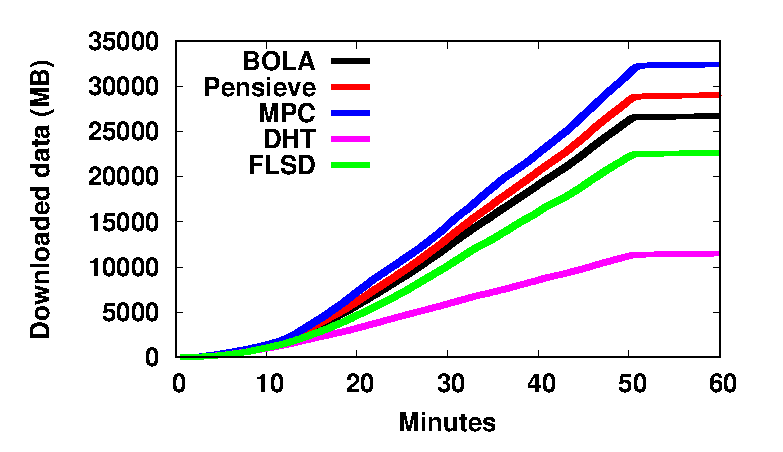
\includegraphics[width=0.49\linewidth]{img/grpbasic/cdnupload_1}
		}
		\subfloat[\label{fig:chap06:cdnuploaded_cnt} Segment downloads from server]{
			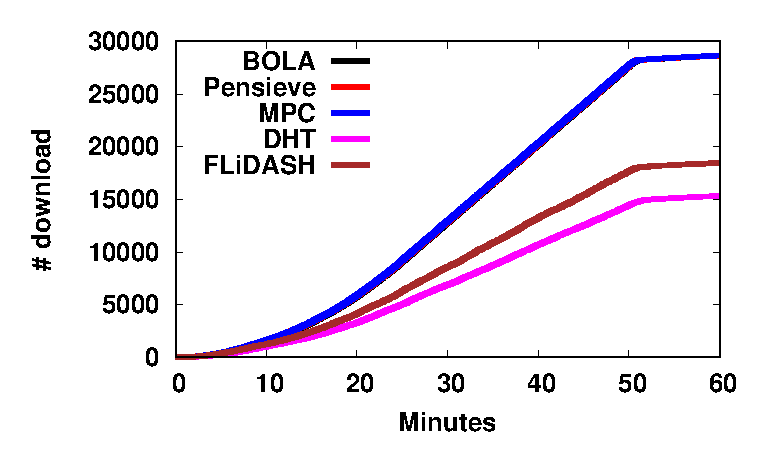
\includegraphics[width=0.49\linewidth]{img/grpbasic/cdnuploadcnt_1}
		}
	\end{center}
	\caption{\label{fig:chap06:cdnuploaded}Direct traffic from the \acs{CDN}: The direct download load from the server is more than the DHT-based approach bus less than other baselines}
\end{figure}
One of the major objectives of {\our} is to reduce the direct traffic from the \ac{CDN} server when multiple co-located players play the same live video. In \fig\ref{fig:chap06:cdnuploaded}, we plot the direct traffic from the content server by different baselines in terms of (a) the total bytes downloaded, and (b) video segments directly downloaded from the content server. We observe that the DHT based system downloads minimum data from the \ac{CDN}. In \our, players are bounded to receive data from its own coalition only, while in case of DHT, a player can share segments with as many players as possible in the complete network. The standalone players need to download all the segments directly from the server. As a consequence, we observe a performance trade-off here between a complete peer-to-peer based approach and the coalition-based approach -- {\our} significantly improves the \ac{QoE} performance while having little increase in the \ac{CDN} traffic overhead. In a nutshell, the proposed approach makes a balance between the \ac{QoE} and the network traffic overhead during live video streaming.

\begin{figure}[!ht]
	\captionsetup[subfigure]{width=0.49\linewidth}
	\begin{center}
		\subfloat[\label{fig:chap06:grp_download}Amount of Data Upload and Download from Individual Players]{
			\includegraphics[width=0.49\linewidth]{img/grpbasic/grpsz_upload_download}
		}
    	\subfloat[\label{fig:chap06:grp_self_dl} Percentage of forceful self-download due to deadline missess]{
    		\includegraphics[width=0.49\linewidth]{img/grpbasic/grpsz_forced_dl}
    	}
	\end{center}
\caption{\label{fig:chap06:grpsz}Effect of Coalition Size -- Large coalitions reduce the CDN load but increase intra-network data consumption and the forceful self-download due to deadline misses}
\end{figure}


\subsection{Impact of Coalition Size}
We next analyze the performance of {\our} in the context of various design choices. First, we check the impact of coalition size on the performance of {\our}\footnote{In all the previous experiments, we have fixed the maximum coalition size to $4$ players}. \fig\ref{fig:chap06:grp_download} shows the amount of data downloaded at each client from the streaming server (\acs{CDN}) and the total amount of upload data from each client indicating the local network traffic that has been used to distribute the downloaded segments among the coalition members. We observe that a large coalition size reduces the download data share among the streaming clients, as the total video data gets distributed among the coalition members. However, we further observe an increase in the upload data share, as each client needs to distribute the individually downloaded video segments to all other clients. However, it can be noted that the download data actually contributes to the network (\acs{CDN}) load, whereas the upload data is over the local network only.

\fig\ref{fig:chap06:grp_self_dl} indicates \textit{the percentage of forceful self-download} with different coalition sizes. We observe that with increasing coalition size, the percentage of forceful self-download drops till coalition size $5$, and then it increases. Ensuring playback synchronization is difficult when the coalition size is either too small or too large. With a very small coalition size, the data download overheads for individual clients increase, and thus, a small variation in the network bandwidth may result in a deadline miss. On the other hand, with a large coalition size, the variation in the instantaneous network bandwidth among the coalition members is more, and therefore the clients having less instantaneous network bandwidth may experience a deadline miss, resulting in a forceful self-download. Therefore, we see that there exists an optimal coalition size ($5$ in our setup) which indeed reduces the forceful self-download thus improves the overall \ac{QoE} by reducing the bitrate variation.    


\begin{figure}[!ht]
	\captionsetup[subfigure]{width=0.49\linewidth}
	\begin{center}
		\subfloat[\label{fig:chap06:grp_dl_share}Download share of a Coalition Member: The average download share of individual players meet the theoretical fair share bound ($y=\frac{1}{x}$)]{
			\includegraphics[width=0.49\linewidth]{img/grpbasic/grpsz_contri_cnt}
		}
      	\subfloat[\label{fig:chap06:grp_fairness}Jain fairness index on QoE acheived among players: Intra-coalition QoE fairness is always good, inter-coalition fairness depends on coalition size]{
      		\includegraphics[width=0.49\linewidth]{img/grpbasic/grpsz_fairness}
      	}
	\end{center}
	\caption{\label{fig:chap06:grp_contri_n_force}Effect of Coalition Size -- Large coalitions reduce the individual download share; the intra-coalition \acs{QoE} fairness index is always good}
\end{figure}

Next, we analyze how the coalition size impacts the total download share among coalition members, indicating the load-fairness of the system. \fig\ref{fig:chap06:grp_dl_share} indicates that a large coalition reduces individual download shares among coalition members. In terms of load-fairness, we observe that large coalitions provide better fairness. We also plot the $y=\frac{1}{x}$ curve which shows the theoretical fair share among the coalition members. It is conforming for us to see that the average load-fairness fits the theoretical fair share. 

To quantify the \ac{QoE} fairness among the coalition members, we measure the Jain fairness index~\cite{jain1999throughput} on the measured \ac{QoE} of the individual players in two categories -- (i) \textit{intra-coalition \acs{QoE} fairness} (fairness among the individual members of a coalition) and (ii) \textit{inter-coalition \acs{QoE} fairness} (fairness among different coalition members). \fig\ref{fig:chap06:grp_fairness} shows that the intra-coalition \ac{QoE} fairness index is always close to $1$, which indicates good fairness among the coalition members in terms of the \ac{QoE} experienced by individual clients of a coalition. However, the inter-coalition \ac{QoE} fairness initially gets reduced with increasing coalition size up to $5$. As different coalitions can play the video in different average bitrates, which has a major contribution to the overall \ac{QoE}, we initially see this drop in the inter-coalition \ac{QoE} fairness. Interestingly, inter-coalition \ac{QoE} fairness increases with a large coalition size, as large coalitions result in less number of coalitions, hence less bitrate variation among different coalitions.

\subsection{Impact on Shared Network Link}
Next we show the results for the topology where the devices are interconnected with the \ac{ISP} gateway through the \ac{LAN} gateway, indicating that they have a common or shared network link. In this case, the shared link becomes the performance bottleneck as all the devices use the same link to download the video segments. In this experiment, we use similar setup as earlier, except that the devices do not have a direct connection to the \ac{ISP}. We perform thorough experimentation to compare the shared link utilization and the video \ac{QoE} of various \ac{ABR} algorithms and \our. In this experiment we use more than $100$ video players that are connected via an internal network or \ac{LAN}, and the players have a high-speed shared Internet connection. We capped the Internet connection speed to $350$Mbps so that all players can not download the maximum quality (bitrate 4.5Mbps) video simultaneously. They have to reduce the quality to avoid buffering. In \fig\ref{fig:chap06:shrd_qoe}, we compare the performance of {\our} and other baselines in terms of the overall \ac{QoE}. We observe that the overall \ac{QoE} for {\our} is better for around $80\%$ of the cases.

\begin{figure}[!ht]
	\centering
	\includegraphics[width=0.75\linewidth]{img/sharedlink/qoe_cdf_1}
	\caption{QoE for shared Internet connection}
	\label{fig:chap06:shrd_qoe}
\end{figure}

We observe another insight that is shown in \fig\ref{fig:chap06:shrd_qoe_flsd} which shows the distribution of the overall \ac{QoE} only for \our. Interestingly, we observe that the \ac{QoE} values jump suddenly after the \ac{CDF} of $0.2$. By close inspection we see that those cases correspond to the scenario when the coalition is not formed. The moment {\our} forms the coalition, the average \ac{QoE} value jumps significantly, and {\our} outperforms other baselines.

\begin{figure}[!ht]
	\centering
	\includegraphics[width=0.75\linewidth]{img/sharedlink/qoe_cdf_flsd}
	\caption{\acs{QoE} jump between independent players and the players in coalition}
	\label{fig:chap06:shrd_qoe_flsd}
\end{figure}


\begin{figure}[!ht]
	\centering
	\includegraphics[width=0.75\linewidth]{img/sharedlink/corenetwork_1}
	\caption{Shared Link Utilization}
	\label{fig:chap06:shrd_link_util}
\end{figure}

Next, we check the shared link utilization as shown in \fig\ref{fig:chap06:shrd_link_util}. Interestingly, we observe that the utilization of the shared link by {\our} is less compared to other baselines. Therefore, this experiment shows that {\our} provides better \ac{QoE} compared to other baselines while utilizing less link bandwidth. Once the coalition is formed, all the players in the coalition gets the best video streaming experience while using far less network bandwidth compared to other baselines. This is a significant improvement in terms of both the cost as well as the performance; the coalition formation can save a significant amount of network bandwidth while providing the best streaming performance to the end users.